%% LyX 2.4.2.1 created this file.  For more info, see https://www.lyx.org/.
%% Do not edit unless you really know what you are doing.
\documentclass[11pt]{article}
\PassOptionsToPackage{natbib=true}{biblatex}
\usepackage[T1]{fontenc}
\usepackage[utf8]{inputenc}
\setcounter{secnumdepth}{5}
\setcounter{tocdepth}{5}
\usepackage{xcolor}
\usepackage{verbatim}
\usepackage{url}
\usepackage{enumitem}
\usepackage{graphicx}
\usepackage{geometry}
\geometry{verbose,tmargin=3cm,bmargin=2cm,lmargin=1.5cm,rmargin=1.5cm}
\usepackage{setspace}
\PassOptionsToPackage{normalem}{ulem}
\usepackage{ulem}
\onehalfspacing

\makeatletter

%%%%%%%%%%%%%%%%%%%%%%%%%%%%%% LyX specific LaTeX commands.
\providecolor{lyxadded}{rgb}{0,0,1}
\providecolor{lyxdeleted}{rgb}{1,0,0}
%% Change tracking with ulem and xcolor: base macros
\DeclareRobustCommand{\mklyxadded}[1]{\textcolor{lyxadded}\bgroup#1\egroup}
\DeclareRobustCommand{\mklyxdeleted}[1]{\textcolor{lyxdeleted}\bgroup\mklyxsout{#1}\egroup}
\DeclareRobustCommand{\mklyxsout}[1]{\ifx\\#1\else\sout{#1}\fi}
%% Change tracking with ulem and xcolor: ct markup
\DeclareRobustCommand{\lyxadded}[4][]{\mklyxadded{#4}}
\DeclareRobustCommand{\lyxdeleted}[4][]{\mklyxdeleted{#4}}

%%%%%%%%%%%%%%%%%%%%%%%%%%%%%% Textclass specific LaTeX commands.
\newlength{\lyxlabelwidth}      % auxiliary length 

\@ifundefined{date}{}{\date{}}
\makeatother

\usepackage[english]{babel}
\usepackage{listings}
\lstset{basicstyle={\ttfamily\small\color{red}},
frame=single,
rulecolor={\color{red}}}
\usepackage[style=authoryear,maxbibnames=9, maxcitenames=2,terseinits=true,giveninits=true,uniquename=false, uniquelist=false]{biblatex}
\renewcommand{\lstlistingname}{\inputencoding{latin9}Listing}

\begin{document}
\title{\texttt{lyxport} documentation}
\author{Mark Bravington, December 2024}
\maketitle

\section{Overview}

The \texttt{lyxport} R package is for exporting LyX to MSWord-{}-{}-
which I sometimes have to do, under duress-{}-{}- and perhaps other
formats. Unlike LyX's built-in ``MS Word Open Office XML'' export,
Lyxport\footnote{I don't approve of starting proper nouns with lower case. Causes more
trouble than it's worth. Sure, software names might be spelt lower-case
for reasonable reasons, but when referring to them, caps read more
naturally in most cases. There's only one Pandoc.} does proper cross-referencing including tables, figures, lists, equations,
appendices, and bibliography; and it sorts out a few other quirks
too. Most of the heavy lifting is still done by Pandoc, as in LyX's
built-in export option. However, Pandoc-{}-{}- wonderful though it
is!-{}-{}- doesn't get everything right even with well-known filters
(as you have probably discovered yourself by now, else you mightn't
be reading this). So Lyxport contains a lot of \emph{my} behind-the-scenes
fiddly code in order to save \emph{you }lots of manual post-fiddling.

The use-case I have in mind is basically my own: you have prepared
a long and lovely paper in LyX that generates a perfect and pretty
PDF. But for some reason you have to submit it to some journal that
insists on miserable misbegotten manuscripts in MSWord. Sigh-{}-{}-
I sincerely feel your pain! There might be several rounds of back-and-forth
between you and the journal, so you reeeally don't want to have to
repeatedly do manual edits of the Word version of an 80\% successful
conversion using an editor you hate. The conversion should look reasonably
decent, citations and cross-refs should all be correct, etc; but journals
always fart around with the appearance of tables etc, so there's no
need to get \emph{every} detail of appearance exactly matching between
PDF and MSWord. And that's the level that Lyxport aims at.

To see the features, open ``examples/lyxport-demo.lyx''. I haven't
tested every LyX feature; it's mostly just stuff I need. More things
might get added.

\subsection{Setup}

Once you've installed the package, run \texttt{lyxprefhack()} to set
things up for direct use from LyX. Then you should see an \textquotedbl MSWord
(lyxport)\textquotedbl{} option in File->Export, and a ``lyxport''
item in LyX's Help menu (this file). You can also see a PDF version
via \texttt{RShowDoc(\textquotedbl lyxport-docu\textquotedbl ,package=\textquotedbl lyxport\textquotedbl )}.

After setup, you won't normally use this package from R yourself;
it will just be invoked from LyX. (The exception is if you want to
use \texttt{requote\_lyx} or any other future ``offline'' support
function— currently that's the only one). However, a keen user could
experiment with the core function \texttt{lyxzip2word }(qv) directly,
e.g. to produce other formats besides MSWord.

\subsection{Do I need to modify my LyX document?}

Currently the only mod you usually need to make to a LyX document,
is adding one line of ERT to define the bibliography style (section~\ref{sec:Bibliographies}).
However, there are general limitations on usable LyX features, some
of which are documented below.

\subsection{Are there are any other useful functions in \texttt{lyxport}?}

The helper function \texttt{requote\_lyx }tries to resolve inconsistent
use of straight quotes, etc; you do have to use that manually from
R, probably only once per LyX file. For example, I used it when creating
this document, which was based on importing plain text files of R
documentation.

\subsection{Versions}

Version 1.0 of Lyport is written for Pandoc 3.5 and Pandoc-crossref
v0.3.18.0. It's quite possible that some of the problems which Lyxport
1.0 deals with, will actually be fixed in future releases of Pandoc.
In that case, the Lyxport fixes might cause other problems..! Of course,
I will try to maintain Lyxport accordingly, but I don't need Pandoc
very often, so I might not get round to it quickly, What I should
perhaps do for future-proofing, is make all the fix options switchable,
and add a single character-string argument to \texttt{lyxzip2word}
which controls all options (it would be disentangled inside \texttt{lyxzip2word}).
Then users could easily-enough hand-modify the LyX Converter, to add
an appropriate version of the argument in the call to \texttt{lyxzip2word}.
But I haven't done this yet.

\section{Bibliographies\label{sec:Bibliographies}}

Citations seem to work fine, ie whatever you specify in LyX for the
PDF version also appears in the Word version— including the different
options for parentheses, commas, etc (which took me a \emph{lot} of
hacking!). However, for the bibliography itself, Pandoc does not understand
\textquotedbl styles\textquotedbl{} in the same way that Biber\slash Biblatex
does (or whatever animal of the Latex zoo it should be; I don't understand
this stuff, and am happy to keep it that way). AFAICS none of the
ways you can alter bibliography appearance in LyX/Latex will be understood.
Instead, you'll need to specify a \textquotedbl CSL style\textquotedbl{}
manually in your LyX source, as follows. First, you will need to get
a suitable CSL file from the internet, eg via \url{https://editor.citationstyles.org/searchByExample}
and store it somewhere (see below for thoughts about where). Second,
you'll need some ERT to tell Lyxport (which will then tell Pandoc)
about the CSL. Here's two options:

%% CSL journal-of-applied-genetics.csl

\bgroup\inputencoding{latin9}
\begin{lstlisting}
%% CSL journal-of-applied-genetics.csl
\end{lstlisting}
\leavevmode\egroup

or

%% CSL ./journal-of-applied-genetics.csl

\bgroup\inputencoding{latin9}
\begin{lstlisting}
%% CSL ./journal-of-applied-genetics.csl
\end{lstlisting}
\leavevmode\egroup

The first— i.e., with no path— is generally better; the CSL file is
available ``globally'' for use by Lyxport on any LyX document. For
that, you need to store the CSL file at the top of your biblio tree,
ie in the folder \textquotedbl <top>\textquotedbl{} where \textquotedbl <top>/bibtex/bib/\textquotedbl{}
contains the actual dot-bib file(s) you are using as biblio sources.
(You would have told your Latex system about your biblio tree at some
point. You might get lucky by trying \texttt{kpsewhich -var-value
TEXMFHOME} in a shell. Or Google.)

The second option, with a ``./'', assumes you store the CSL file
``locally'', ie in the same folder as the LyX document that's mentioning
it. In that case, you'll also need to insert the file as a Verbatim
child document inside a Comment, like this:

\begin{comment}
\verbatiminput{journal-of-applied-genetics.csl}
\end{comment}

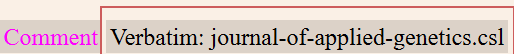
\includegraphics{fake-verbatim}

The Comment prevents the contents of the CSL file from appearing in
the rendered document (eg in PDF form), but the mention of a child-document
tricks LyX into including the CSL file during File->Export->Lyx-zip
(which is done automatically for you, as the first step in conversion
to MSWord etc). (If I'd realized how Comments actually work, I would
have used that instead of ERT for CSL-specification in the first place.)

If you specify several CSLs with that \texttt{\%\% CSL} mechanism,
then only the final one will be used.

\subsection{Capitalization}

Biblatex/Biber seem to take account of capital letters without having
to wrap them in \{\}, but MSWord and CSS don't, so that references
which work fine with the former sometimes don't with the latter, unless
tweaks are made. \texttt{lyxzip2word()} therefore contains code to
forcibly capitalize references (i.e., changing the entries in a copy
of the bibliography) where it looks like the user meant it. (Citations
where the first word starts lower-case, e.g. for referring to a piece
of Software, are also kept that way.) This might not be exactly the
behaviour that \emph{you} want, but \emph{I} sure need it! So, you
have to be careful to get your original biblio entries right; Capital
in the database will mean Capital in the MSWord output, too.

\subsection{Same author, multiple names}

In a dot-bib file, the same author can appear with slightly different
names in different papers: \textquotedbl A. Psmith\textquotedbl ,
\textquotedbl Alan Psmith\textquotedbl , \textquotedbl Alan B.
Psmith\textquotedbl , \textquotedbl A. Bertram Psmith\textquotedbl ,
and so on. If you are not careful, your citations can come out funny
as a result. For example, you might see \textquotedbl Psmith et al.
(1999)\textquotedbl{} but \textquotedbl A.B. Psmith (2004)\textquotedbl{}
even though Alan Bertram is the only Psmith you are citing. With Biblatex
and PDFs, you can suppress such nonsense via \texttt{uniquename=false}
and \texttt{uniquelist=false}. But with CSL and MSWord etc, it seems
to be harder-{}-{}- like everything, actually. \texttt{lyxzip2word()}
sorts this out, rather forcibly, by calling \texttt{tidy\_initials()}
for you. The default behaviour is ``lumping'', so that ``A.B. Psmith''
and ``A. Psmith'' will be assumed to both be ``A.B. Psmith'' (but
clear contradictions still won't be). You can turn that off via:

%% tidy_initials FALSE

\bgroup\inputencoding{latin9}
\begin{lstlisting}
%% tidy_initials FALSE
\end{lstlisting}
\leavevmode\egroup


\subsection{DIY bib-hacking}

The CSL website I link to above is terrific, but sometimes you just
can't find a CSL that really does what you want; and editing an existing
style seems incredibly difficult\footnote{I did try tried. And I tried again. And I gave up. There are limits
even to \emph{my} obstinacy.}. One \emph{desperate} option might be to temporarily hack Lyxport's
temporary copy of your own biblio file so that it Looks Nicer (because
you don't want to change your original bib file). For example, I wanted
one particular institution to always be abbreviated, even though the
bib file has it spelt out in full. So you can add your own R function
to do that, along the lines below (it must be embedded in a Comment).
The sole argument of the function should be a character vector (the
text from the file), which your function should modify and return.

\begin{comment}
%% Bibhack
function( bibbo){
  insti <- grep( '^ *[Ii]nstitution *=', bibbo)
  IWC_full <- '.nternational +.haling +.ommission'
  iwc <- insti[ grep( IWC_full, bibbo[ insti])]
  bibbo[ iwc] <- gsub( IWC_full, 'IWC', bibbo[ iwc])
return( bibbo)
}
%% End Bibhack
\end{comment}

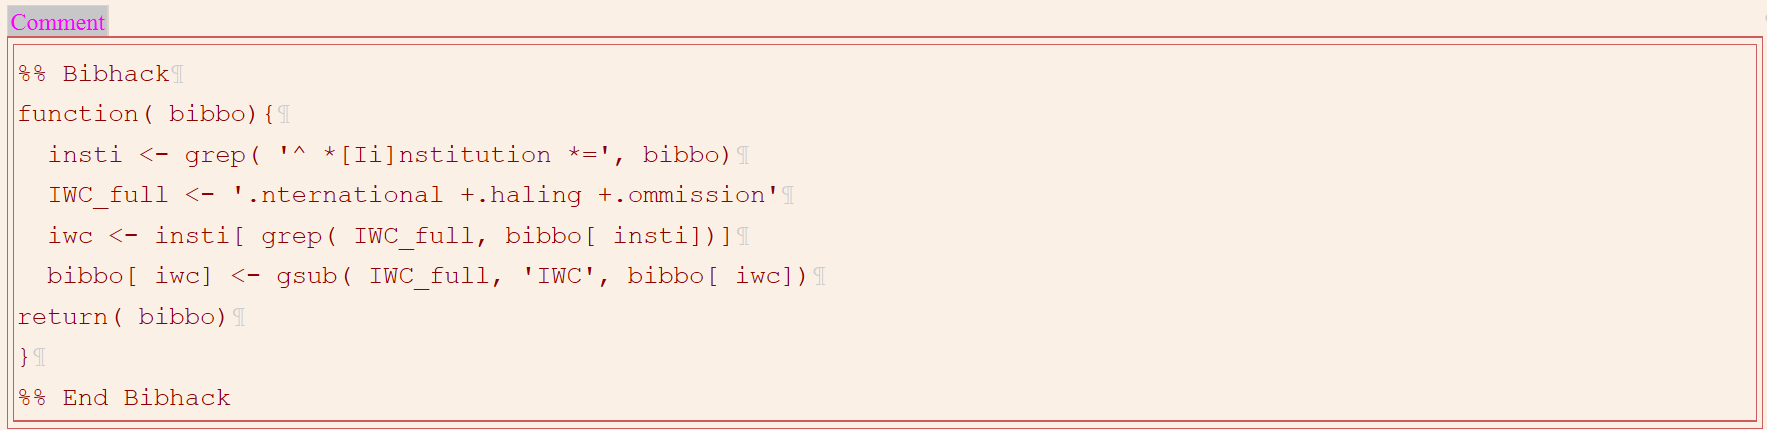
\includegraphics{fake-bibhack}

\section{Other formats}

My requirement is for MSWord, so that's what I've concentrated on.
Things might or might not work in other formats; almost all the work
in Lyxport is in generating a nice native-Pandoc document, and the
final export step is just up to Pandoc, so there is a good chance
other output formats will work at least reasonably. You can experiment
inside R with the \texttt{outext} and \texttt{panoutopts} arguments
of \texttt{lyxzip2word}. First, you will need to export your test
document from LyX as a ``LyX archive'' (lyxzip). 

FWIW I personally would prefer to use ODT rather than MSWord if I
could (since ODT is open-source and the MSWord \emph{program} can
import ODT), but unfortunately LibreOffice's maths importing is broken
(as of v7.6 and for some time before that). {[}One example: the vertical
bar, which I use extensively for conditional probability. But there's
other things too.{]} \textquotedbl Barring\textquotedbl{} that for-me-deal-breaking
limitation, 'lyxzip2word' can export quite nicely to ODT, except figure
sizes are not respected-{}-{}- whether that's down to Pandoc's ODT
writer, or to a limitation of ODT itself, I don't know. You'd need
to manually resize all the figures within LO :/ Maybe there's an option
in native Pandoc to specify figure sizes, in which case I could probably
add code to do that-{}-{}- but there's no point unless the ODT maths
things get fixed.

\section{How it works}

In LyX, there needs to be a new \textquotedbl File Format\textquotedbl{}
(in Preferences) which is an alias for the existing MSWord format.
(The same would apply to any other desired type of output.) Then there
needs to be a \textquotedbl Converter\textquotedbl{} from \textquotedbl Lyx-zip
(archive)\textquotedbl{} format to the new alias. When you pick \textquotedbl File->Export->{[}new
format alias{]}\textquotedbl , LyX will realize that the only way
to produce the new format is to first export to Lyx-zip (producing,
yes, a zip file), then run the new Converter. The latter launches
R, and runs \texttt{lyxport::lyxzip2word} which does everything else,
starting from that zip file. \textquotedbl Everything else\textquotedbl{}
means: LyX -> Latex -> pre-process -> Pandoc-tex-to-native -> post-process
-> Pandoc-native-to-MSWord-or-other.

This package is very effective despite \emph{my} limitations: I don't
understand Pandoc's internal document structure, I have zero wish
to learn new programming languages or arcane file formats, and I have
a pretty limited understanding of Latex-{}-{}- much of the point of
LyX being to avoid having to remember all the Latex gruesome details!
However, the good news is that LyX exports a highly structured and
limited form of Latex (unless you insert really nasty ERT...) which
makes it easy to \textquotedbl partially parse\textquotedbl{} the
file using 'grep' etc to find constructs that need attention. Similarly,
Pandoc exports a highly-structured \textquotedbl native\textquotedbl{}
format which IMO is much easier to partially-parse than JSON-{}-{}-
for example, indentation is highly consistent, so I can usually find
the range of lines to 'gsub' etc by matching indentation size. Then
I monkeyed around (a lot) until things worked.

Because I rely on LyX's specific and tidy structuring of its Latex
exports, 'lyxzip2word' simply won't work on generic Latex documents.

In slightly more detail, the steps are:

- From inside LyX, LyX exports to LyX-zip, containing all Lyx source
files and all graphics in a single file.

- LyX calls a converter script to convert to target format (an \textquotedbl alternative
MSWord\textquotedbl ), which launches R and runs 'lyxzip2word'.

See 'lyxzip2word' for more detail on the actual conversion steps.

\section{Pandoc options}

Pandoc uses an output-format-specific \textquotedbl template\textquotedbl{}
or ``reference-doc'' to control some aspects of its output, eg fonts.
See \texttt{https://pandoc.org/chunkedhtml-demo/6-templates.html}
and\texttt{https://pandoc.org/MANUAL.html\#option-{}-reference-doc}.
You might want to change the template; for example, Pandoc's default
choices for MSWord \textquotedbl bold\textquotedbl{} looks pretty
weird to me. The template/reference-doc also seems to be the place
where you set features such as line- and page-numbering. (I have included
an example, ``iwc-pandoc-reference.docx'', which started from the
default that Pandoc describes in the above links; note that, to have
any effect, you must edit the \emph{style} of an item, not the appearance
of the item itself.) Then you must also tell Pandoc which template
to use, by adding ERT like this (which again will not be visible in
the PDF or DOCX version):

%% Pandoc reference-doc ./iwc-pandoc-reference.docx
%% Pandoc template zzz-format-reference.zzz

Some output formats, including MSWord, require a ``reference-doc'',
while others want a ``template''; so, use the appropriate word.
As you see, you can specify different ones for different formats,
which will be automatically selected depending on which Converter
you invoke (assuming you have set up LyX Converters for more formats
than MSWord). File location works the same way as CSS bibliography
styles. No path means top of the TEXMF tree, ``./'' means same folder
as the document, in which case you need to add something like this
(again, invisible in PDF and DOCX):

\begin{comment}
\verbatiminput{iwc-pandoc-reference.docx}
\end{comment}

Try to avoid filenames with spaces— here, and everywhere else!

\section{Limitations}

There are probably lots more than this. The list is in two parts,
of which the first seems fairly permanent— it's structural stuff.
\begin{itemize}
\item Labels must start with the right prefix for the thing they are labelling:
\textquotedbl tab:\textquotedbl{} for table-floats, \textquotedbl fig:\textquotedbl{}
for figure-floats, \textquotedbl eq:\textquotedbl{} for equations,
\textquotedbl sec/subsec/par:\textquotedbl{} for sectioning, and
\textquotedbl enu:\textquotedbl{} for lists. LyX will do this automatically
for you when you set up a label, unless you perversely force it not
to; so, don't do that.
\item In order to \textquotedbl count\textquotedbl , tables \& figures
have to be in floats with labelled captions. Each float can contain
several actual tables or figures, but only one label. Requiring a
label is reasonable; how else would you alert the reader to the existence
and role of the table inside the main text?! Numbered sections and
numbered equations don't need labels, unless they are cross-referenced.
\item Figures: No absolute paths. (Otherwise, Lyx-zip-export uses lots of
subfolders and I can't find the files.) I'm not sure about relative
paths that go \textquotedbl upwards\textquotedbl{} either (eg \textquotedbl ../sister/image.png\textquotedbl ).
\item Equations inside tables won't be labelled.
\item TOC \& lists of Figures, etc. Since those are page-number-specific,
they won't translate 100\% between Latex \& MSWord anyway.
\item Multi-page figures using subfloat/ContinuedFloat \emph{do }work, but
you shouldn't put anything in the subfloat captions per se because
they will not be printed (deliberately, Becoz Reasons). However, you
can put things in the main caption of each continuation float.
\item Your local ``layouts'' (LyX modules) won't be available unless you
copy them somewhere else; see section~\ref{sec:The-LyX-userdir}.
This is a LyX bug that might get fixed.
\end{itemize}
Overall, the biggest limitation is Pandoc's Latex reader, but there
are other problems too. For example: the \textquotedbl cases\textquotedbl{}
environment gets spurious RH paren on export, LibreOffice/ODT maths
has got problems, ... Anyway, for the second part of the list, here
are some current limitations that I \emph{might} fix in future:
\begin{itemize}
\item No Boxes (yet). In particular, resizebox and presumably its friends
don't work (unfortunately, since I often use them to get tables to
fit). Perhaps I should add code to delete them from the intermediate
Latex files, so that at least something comes out.
\item Table column widths are ignored.
\item Only one Bibliography is produced.
\item Equation numbering is either unsectioned (1, 2, 3 etc) or uses \textquotedbl section\textquotedbl{}
as the prefix (1.1 etc). In principle it should also accept \textquotedbl chapter\textquotedbl{}
or \textquotedbl part\textquotedbl{} for the prefix. Perhaps it should
also allow user-specified arbitrary prefixes.
\item Equations, Figures, and Tables in Appendices are numbered (A1,A2,...,B1,B2)-{}-{}-
no choice (and it's my preferred way). ?Should I allow user-specced
Apx encoding, eg S1, S2 instead of A, B? I don't know how to enforce
any of this in LyX/Latex anyway.
\item Lists always use LyX's default numbering hierarchy, eg 1-a-i-A. And
there's no support for Enumerate-Resume yet.
\item Citations are all author\slash year, rather than square-brackety.
You can control citation appearance in the usual way.
\end{itemize}

\section{Requirements}

This all needs Pandoc, ImageMagick (which at least on Windows should
be installed automatically inside LyX's folder structure), and, of
course, LyX itself.

The folders for the executables of Pandoc, LyX, and Rscript should
be in the system path. If they aren't normally, then you can tell
LyX to set them up automatically just within each LyX session, via
\textquotedbl Tools->Preferences->Paths->PATH prefix\textquotedbl .

I am going to assume that R\_LIBS\_USER and so on correctly set the
libraries, ie the path(s) to R package folders.

\section{The LyX userdir\label{sec:The-LyX-userdir}}

There's a bug in LyX 2.4.2.1 (at least) which means that, if you have
a personal LyX userdir (which surely everyone does), it can't be made
visible to LyX during the export operation. Normally this doesn't
matter, because the userdir is mostly about interactive session stuff
such as keybindings, but it does mean that any special modules in
your \textquotedbl <userdir>/layouts\textquotedbl{} folder will not
be visible. If you can't live without them, you will just have to
copy them to your \textquotedbl <LyX-system-dir>/layouts\textquotedbl{}
folder.

For those who really want to know (be warned: do you really?), the
problem is this: \texttt{lyxzip2word} needs to call a standalone LyX
instance in order to export a Latex version of the source. (Most of
the needed files-{}-{}- the LyX source itself, any include-files,
graphics-{}-{}- are first exported into the Lyx-zip archive which
is produced automatically, but the Latex version needs to be exported
separately.) There is a handy CLI option \textquotedbl lyx -{}-export
latex <blah>\textquotedbl{} for that. Unfortunately, the latter seems
to fall over if the userdir is set, either on the invocation line
via \textquotedbl -userdir <blahblah>\textquotedbl , or via the
\textquotedbl LYX\_USERDIR\_24x\textquotedbl{} envar. Then LyX will
crash with a SIGSEGV (and exit code 11 in Windows). When LyX calls
Rscript, it \emph{sets} that envar first-{}-{}- which is normally
good, coz it means that a converter could look at any userdir settings.
However, when Rscript then calls LyX again, it will crash. So Rscript
(ie \texttt{lyxzip2word}) has to \emph{unset} that envar before calling
LyX, which means that the second instance of LyX cannot know about
your modules. You were warned!

\section{FAQ}
\begin{description}
\item [{Q:}] \emph{I have exported my beautiful PDF to MSWord and now it
looks like {*}{*}{*}{*}. What can I do about that?}
\item [{A:}] Well, yes, that's MSWord for you. 
\item [{Q:}] \emph{Why did you use R rather than writing a series of }Pandoc\emph{
filters in SDGL to translate FSDOIG format, like you're supposed to?}
\item [{A:}] Because I know R, and I have no interest in learning SDGL
nor figuring out the intricacies of FSDOIG format. Also, modern R
is really good for regexy manipulations-{}-{}- people often don't
realize that. If you don't already have R (which I expect many LyX
users will), then it's not hard to install.
\item [{Q:}] \emph{You clearly had to fix lots of issues. Why didn't you
report them as bugs and wait for someone else to sort them out, like
a logical systematic person would?}
\item [{A:}] Because I needed this for my own purposes, and fairly quickly.
Other people are busy, and might not have the same view of what constitutes
a \textquotedbl bug\textquotedbl{} or \textquotedbl something worth
fixing\textquotedbl{} as I do. Like people say: ``if you want something
done properly, do it yourself''. That said, I really ought to get
round to reporting the bugs at some point-{}-{}- but reporting bugs
is quite time-consuming. I tried lots of Pandoc options involving
\texttt{citeproc}, \texttt{eqnos}, \texttt{crossref}, and writen options,
and just could not get things to behave, but I didn't record the failures
in detail. If you try exporting ``eqntest1.lyx'' with LyX's built-in
MSWord exporter, you'll get some idea...
\item [{Q:}] \emph{Your approach based on counting indents etc is terribly
fragile and Offensive To Logic. It is much better to build entire
parse trees and then transmogrify the glorts using percortical DeMoivre
contextual fermions.}
\item [{A:}] Errr, maybe so. But my approach \emph{works}, and it works
\emph{now}, and \emph{I} need it now!
\item [{Q:}] \emph{Hmmm, I prefer to write all my documents in raw Latex
because it is the Only True Way for ninth-level ninjas like myself;
GUIs like LyX are for lesser mortals, monotremes, slime moulds, etc.
However, I reluctantly concede that Lyxport does quite a good job
of exporting to MSWord, and I note that it actually starts from a
Latex file (as exported by LyX). Can I make use of it on my own Latex
files?}
\item [{A:}] How very gracious of you. But to answer your question: no,
not directly on general Latex files. There might be other tools Out
There for that. Lyxport relies on the tightly-structured flavour of
Latex exported by LyX. Your only chance would be to import your Latex
into LyX, then export. It \emph{might} all work, but expect pain.
\item [{Q:}] \emph{Is this really a FAQ?}
\item [{A:}] Am I really Mickey Sodding Mouse?
\end{description}

\end{document}
